\section{Robotat}

En la Universidad del Valle de Guatemala se cuenta con el ecosistema Robotat descrito
 en \cite{perafan_montoya_robotat_2022}, que consiste en un ecosistema formado por una red
 de comunicación WiFi, así como también un sistema de captura de movimiento OptiTrack, el 
 cual emplea un total de seis cámaras. Adicionalmente Robotat cuenta con una antena inteligente la cual
 combina la información obtenida por medio del sistema de captura de movimiento, con información dada
 por una unidad de medición inercial de forma que es posible el intercambio de información entre agentes
 mediante comunicación inalámbrica.

\begin{figure}[H]
        \centering
        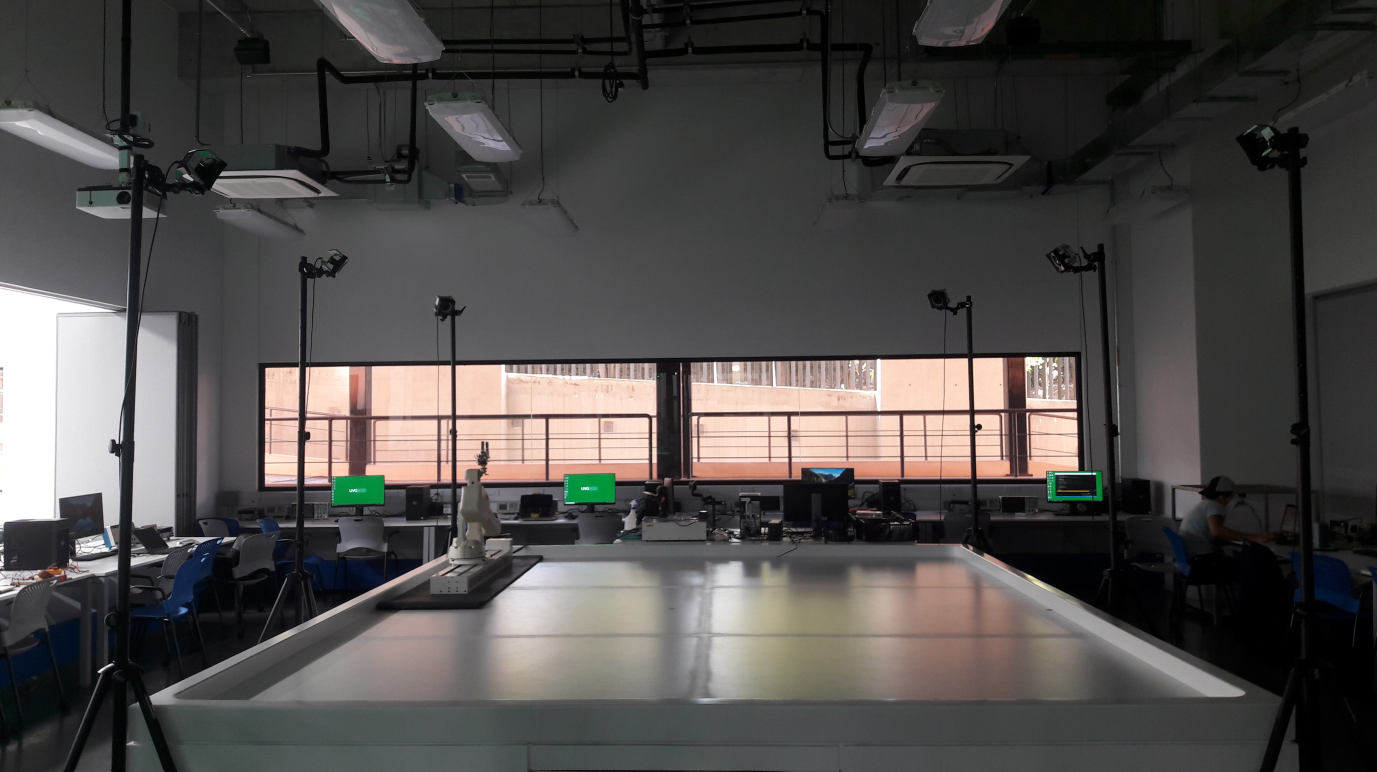
\includegraphics[scale=.4]{imagenes/robotat.png}
        \caption{Ecosistema Robotat \cite{perafan_montoya_robotat_2022}}
        \label{fig:robotat}
\end{figure}

\section{Robotarium del Georgia Institute of Technology}

El Robotarium es un proyecto diseñado por \textit{Georgia Institute of Technology}, con la finalidad
de tener una plataforma \textit{multi-robot} que pueda ser accedida de forma remota y de fácil acceso al público.

Este proyecto es presentado en \cite{wilson_robotarium_2021} como una herramienta de propósitos educacionales
así como para aplicaciones de robótica avanzada. 
En el prototipo inicial del Robotarium, los agentes robóticos utilizados son
GRITSBot que, para asegurar su autonomía se encontraban equipados con un sistema de carga inalámbrica,
 el cual tenía bobinas de inducción orientadas hacia el suelo
de forma que los GRITSBot eran recargados por medio de transmisores instalados en el suelo. Sin embargo, este sistema
contaba con la desventaja que para maximizar la eficiencia al cargar,  era necesario que los 
transmisores y las bobinas instaladas en los agentes estuvieran lo más cerca posible. Debido a las técnicas
 de fabricación existía la posibilidad de que los robots montados se arrastraran en la superficie,
o bien se encontrarían a una distancia que impidiera la carga.

Debido a los inconvenientes mencionados anteriormente el sistema de carga fue reemplazado por unidades de transmisión
inalámbricas colocadas en los muros de la arena del Robotarium, así como también unidades receptoras instaladas en la 
parte trasera de los GRITSbot. Con este nuevo diseño las unidades de carga pueden ser manufacturadas de forma
 mas rápida, utilizando corte láser, y cargadores inalámbricos comerciales. Adicionalmente al estar los cargadores
 montados en el muro se tiene un proceso de carga más fiable al permitir un contacto casi directo con los robots,
 sin la necesidad de colocar los receptores cerca del suelo \cite{wilson_robotarium_2021}. 

 \begin{figure}[H]
    \centering
    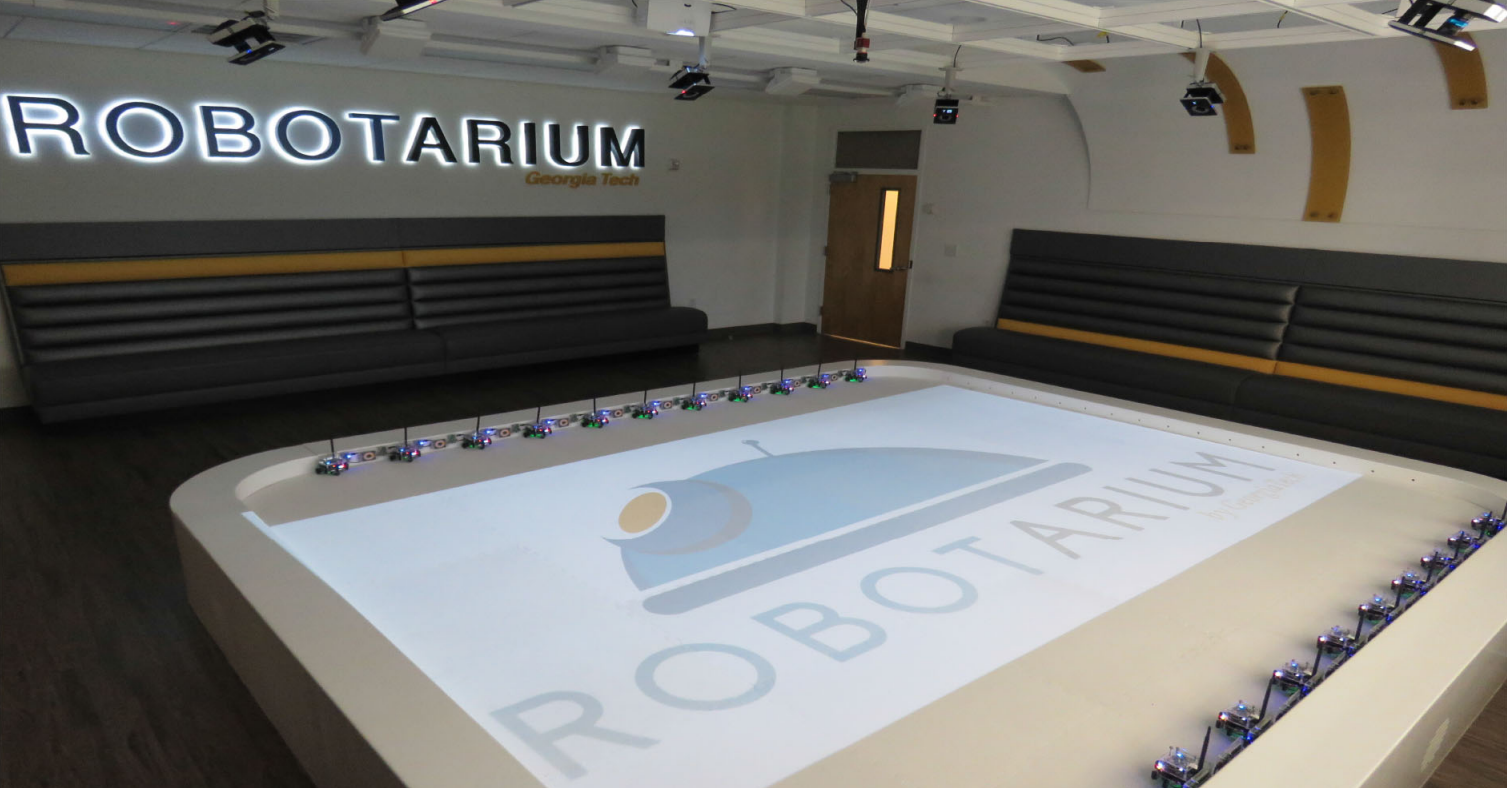
\includegraphics[scale=.4]{imagenes/Robotarium.png}
    \caption{Arena del  Robotarium  \cite{wilson_robotarium_2021}}
    \label{fig:robotarium}
\end{figure}

\section{Cargadores de baterías multiquímica}
En la actualidad para muchas aplicaciones es de gran importancia el uso
baterías para tener movilidad y autonomía, de igual forma también es indispensable
el desarrollo de sistemas de carga que sean eficientes. En \cite{cleveland_developing_2015}
se presenta el desarrollo de un cargador multiquímica de baterías programable, el cual se 
encuentra basado en el circuito integrado MCP19111 de Microchip, que es un
\textit{Digitally-Enhanced Power Analog Controller}, este, a grandes rasgos es un controlador el cual
contiene lazos de control analógicos con interfaces digitales para el monitoreo y manipulación de parámetros
de forma que sea posible el ajuste del sistema mientras se encuentra en operación pudiendo mejorar el rendimiento
significativamente.  

En el \textit{Massachusetts Institute of Technology} se desarrolló el sistema WafferSat el cual  es un satélite que emplea 
sistemas microelectromecánicos para reducir su tamaño. En \cite{zapien_electrical_2020} se explica el uso del controlador de 
carga BQ25703A, manufacturado por Texas Instruments para el diseño de seguidor de máximo punto de potencia (MPPT, por
sus siglas en inglés) el cual es empleado en el WafferSat para el sistema de carga solar de baterías de polímero
 de iones de litio (LiPo).

\section{Estación de carga inalámbrica para UAV}

En \cite{junaid_design_2016}, se presenta el diseño de una estación de carga inalámbrica para UAV
(Vehículo Aéreo No Tripulado, por sus siglas en inglés). Este proyecto surge debido a que los multicópteros,
 en general, tienen una demanda alta de potencia, lo que limita su tiempo de vuelo, especialmente en el caso
de aquellos de pequeñas dimensiones. Para lograr que estos multicópteros puedan operar durante períodos prolongados,
resulta necesario recargar sus baterías, lo cual generalmente requiere intervención humana directa. En el desarrollo
de esta plataforma de carga, se utilizó la placa DFRobot Leonardo, basada en el microcontrolador ATmega32u4, que
incluye un conector Xbee integrado para permitir la comunicación inalámbrica con módulos Zigbee. En cuanto a la transmisión
de energía hacia el multicóptero, se empleó un sistema de carga inalámbrica, el cual fue prototipado utilizando placas perforadas.
 El sistema diseñado logró alcanzar una eficiencia máxima del 63.4\% \cite{junaid_design_2016}.

\begin{figure}[H]
    \centering
    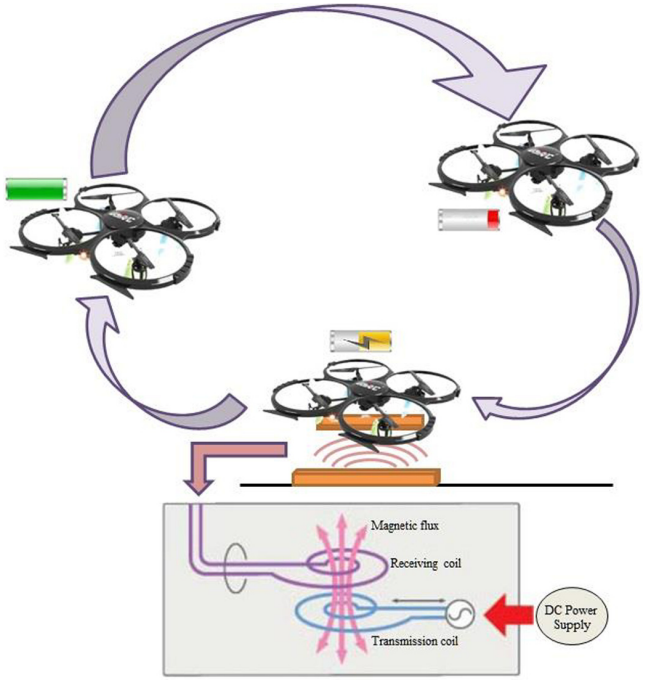
\includegraphics[scale=.4]{imagenes/AUV.png}
    \caption{Concepto de la solución propuesta \cite{junaid_design_2016}}
    \label{fig:1}
\end{figure}

\begin{figure}[H]
    \centering
    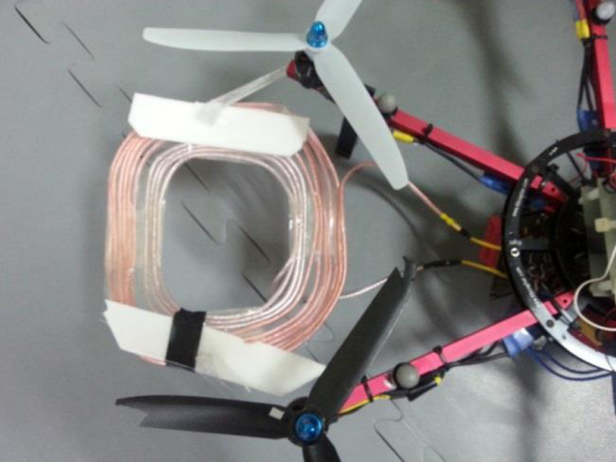
\includegraphics[scale=.4]{imagenes/cuadracoptero.png}
    \caption{Hexacóptero junto con la bobina receptora \cite{junaid_design_2016}}
    \label{fig:hexacoptero}
\end{figure}




